% -*- root: ../Presentation.tex -*-
\section{Hiding Data in JPEG Images}
%PNG SECTION
\begin{frame}{Hiding Data in JPEG Images}{}
	\begin{minipage}[0.5\textheight]{\textwidth}
		\begin{columns}[T]
			\begin{column}{0.5\textwidth}
				\begin{itemize}
					\item In PNG images all pixels can be changed separately
					\item Enables the use of methods such as LSB with a very high payload
				\end{itemize}
			\end{column}
			\begin{column}{0.5\textwidth}
				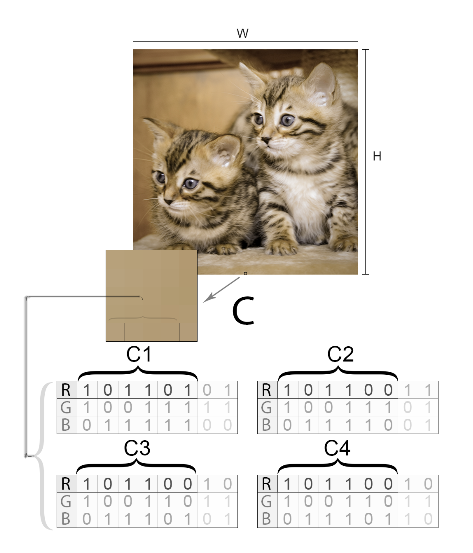
\includegraphics[width=\textwidth]{figures/pngImage.png}
			\end{column}
		\end{columns}
	\end{minipage}
\note{
	\begin{itemize}
		\item Kontrol over hver enkelt pixel, på samme måde som et BMP billede.
		\item Information vi kan få igennem: $\frac{H\cdot W}{8}$ bytes / tegn hvis ASCII (gange to i vores program)
		\item Fast mængde information, med sådanne teknikker
	\end{itemize}
}
\end{frame}
%JPEG SECTION
\begin{frame}{Hiding Data in JPEG Images}{}
	\begin{minipage}[0.5\textheight]{\textwidth}
		\begin{columns}[T]
			\begin{column}{0.5\textwidth}
				\vspace{.56mm}
				\begin{itemize}
					\item JPEG images are divided into MCUs
					\item Further divided into 8x8 blocks
					\item After performing DCT and quantization there is an 8x8 block of integers
				\end{itemize}
			\end{column}
			\begin{column}{0.5\textwidth}
				\begin{center}
					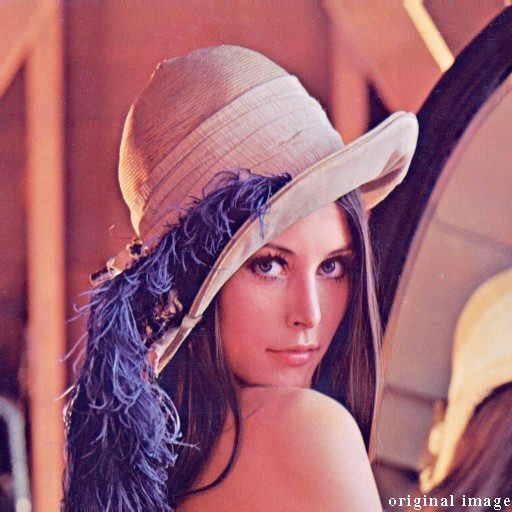
\includegraphics[width=.5\textwidth]{figures/lena_color.jpg}
				\end{center}
				{\tiny \begin{table}[]
				\centering
					\begin{tabular}{|c|c|c|c|c|c|c|c|}
					\hline
					-26 & -3 & -6 & 2  & 2  & -1 & 0 & 0 \\ \hline
					0   & -2 & -4 & 1  & 1  & 0  & 0 & 0 \\ \hline
					-3  & 1  & 5  & -1 & -1 & 0  & 0 & 0 \\ \hline
					-3  & 1  & 2  & -1 & 0  & 0  & 0 & 0 \\ \hline
					0   & 0  & 0  & 0  & 0  & 0  & 0 & 0 \\ \hline
					0   & 0  & 0  & 0  & 0  & 0  & 0 & 0 \\ \hline
					0   & 0  & 0  & 0  & 0  & 0  & 0 & 0 \\ \hline
					0   & 0  & 0  & 0  & 0  & 0  & 0 & 0 \\ \hline
					\end{tabular}
				\end{table}
				}
			\end{column}
		\end{columns}
	\end{minipage}
	\note{
		\begin{itemize}
			\item Meget matematisk billedeformat
			\item Ingen adgang til de enkelte pixels, da de regnes som en fælles block
			\item Starter med en 16x16 block, da vi bruger 4:2:2 sampling $\rightarrow$ 6 8x8 blocks (4 Y, 1 Cb, 1 Cr) $\rightarrow$ DCT $\rightarrow$ quantization $\rightarrow$ huffman encoding $\rightarrow$ skrives til filen (Zero-length entropy).
			\item JPEG encoder lavet til formålet
		\end{itemize}
	}

\end{frame}


\subsection{Techniques}
\begin{frame}{Techniques of Hiding Data in JPEG Images}{}
	\begin{itemize}
		\item<1 -> A naive approach to hiding data is simply appending the clear text to the image
		\item<2 -> A better approach is to trick the decoder with APP$_n$ segments
		\item<3 -> Maybe try to use the LSB method on DCT tables?
		\begin{itemize}\item<4 -> On thumbnail?\end{itemize}
		\item<5 -> A Graph-theoretic approach
	\end{itemize}
	\note{
		\begin{itemize}
			\item Skriv efter EOI marker, simpelt men åbenlyst
			\item Falske APP$_n$ segmenter, snyder en decoder men ikke et system eller person der leder efter data.
			\item LSB giver fast mængde data, men gør billedet meget stort, og tydeligør at der er noget der ikke er som det skal være, thumbnail god ide, men meget ekstra data
			\item Grafteori er det mest avanceret, men måske det mest skjulte
		\end{itemize}
	}
\end{frame}
